\documentclass[12pt]{article}
\usepackage{a4wide}                        
\usepackage{graphics}
\usepackage{graphicx}
\usepackage{color}
\usepackage{alltt}
\usepackage[utf8]{inputenc}
\usepackage[portuguese]{babel}               
\usepackage{latexsym}
\usepackage{hyperref}
\newenvironment{code}                    
{\textbf{
} \hspace{1cm} \hrulefill \\ 
\smallskip 
\begin{center}
\begin{minipage}{0.9\textwidth} 
\begin{alltt}\small}
{\end{alltt}
\end{minipage}
\end{center}
\hrule\smallskip
}
\renewcommand*\rmdefault{iwona}


% Definição do titulo do documento 
%\begin{

\title{\textsf{Programação Orientada aos Objetos} \\
\begin{tabular}[t]{c}
{\small LCC}
{\small Universidade do Minho} \\
{\small Ano Letivo 2015/2016}  \\
{\small ImOObiliária | Trabalho prático} \\
\end{tabular}
}

\author{\small
\\
\\
Grupo 5
\begin{tabular}[t]{lll}
62134 & LCC  & Sérgio Oliveira \\
66698 & LCC  & Carlos Silva\\
\end{tabular}
}

{\begin{document}

\begin{figure*}[b]
        \centering

\includegraphics[scale=0.3]{000.png}	 

\includegraphics[scale=0.2]{001.png}
\end{figure*}


%-------------------- Inicio do Documento ----------------------------------------------------------------------

\maketitle                                            % instrução para incluir o titulo
\pagebreak
                                                        % no documento.

\section{Introdução}

Nós somos o Sérgio Oliveira e o Carlos Silva, do grupo 18 da cadeira de Programação Orientada aos Objetos. Temos como objetivo construir uma interface (gráfica ou terminal, a escolha é nossa) de gestão de uma imobiliária.


%\begin{figure*}[!b]
     %   \centering
%\includegraphics[scale=0.38]{}
%\end{figure*}
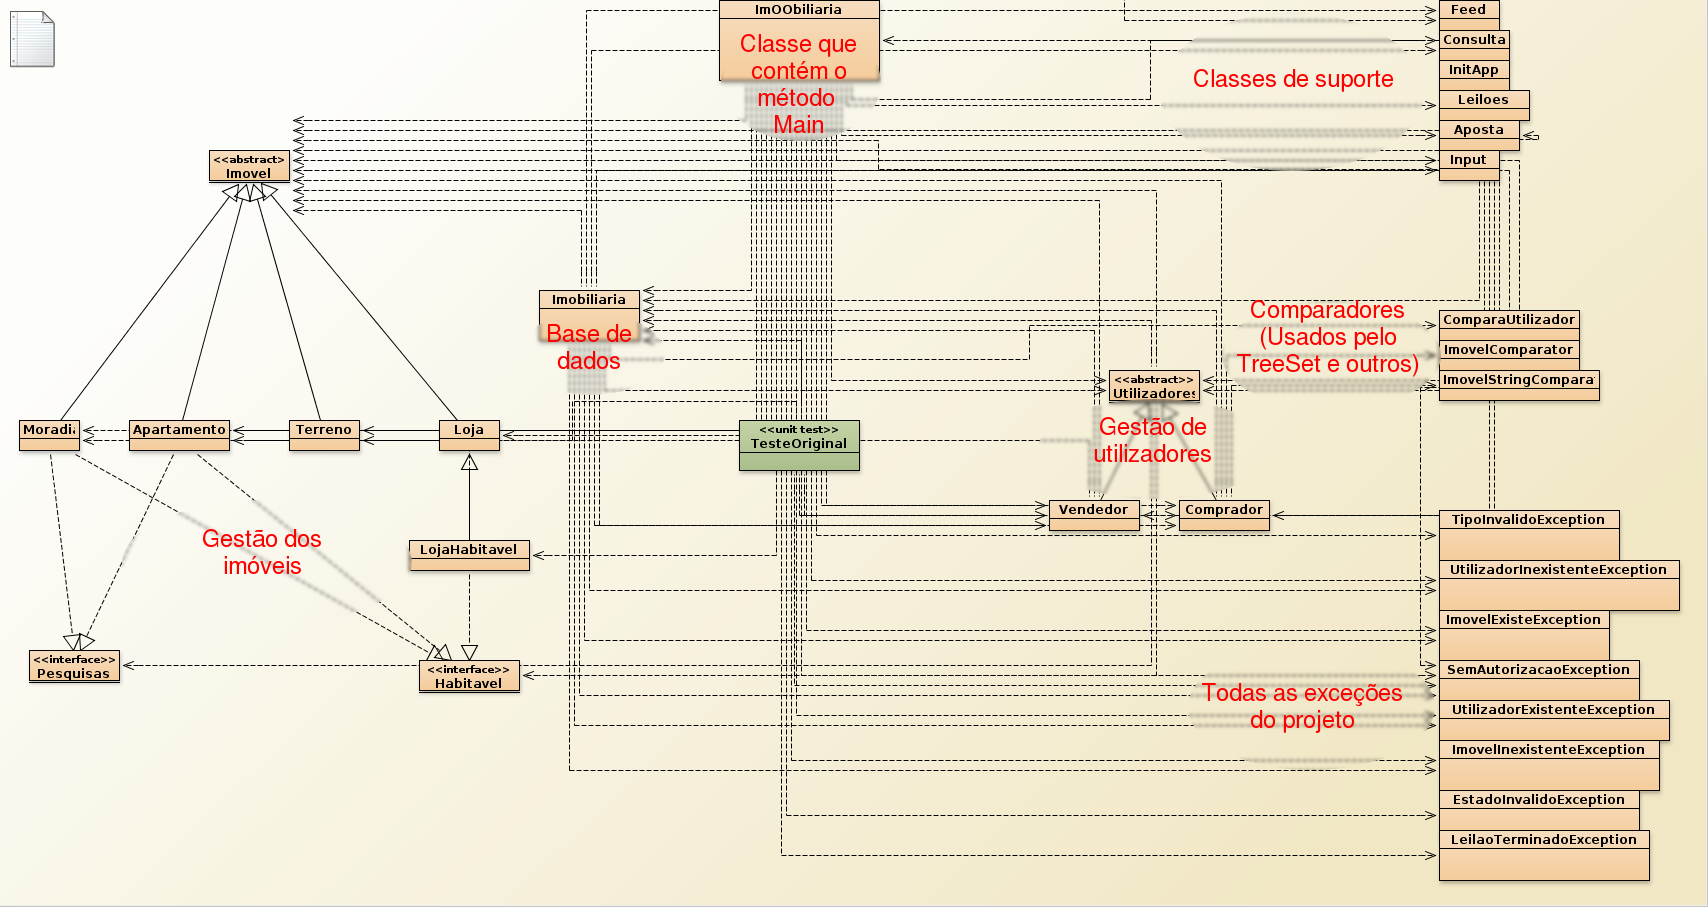
\includegraphics[scale=0.27]{004.png}	
\pagebreak

\section{Primeiras classes}

\textbf{JAVA API}
\newline

Vamos começar com a parte mais obvia de qualquer projeto.\\
Para conseguirmos compilar este programa, recorremos a algumas bibliotecas da Interface de programação de aplicações do JAVA.\\
Essas bibliotecas são as seguintes:
\newline

\begin{code}
java.util;
java.io;
java.lang;

\end{code}
~\\

Fizemos grande parte deste projeto no programa BlueJ mas devido a algumas limitações deste programa, começamos a tomar outros rumos.
\newline
\newline
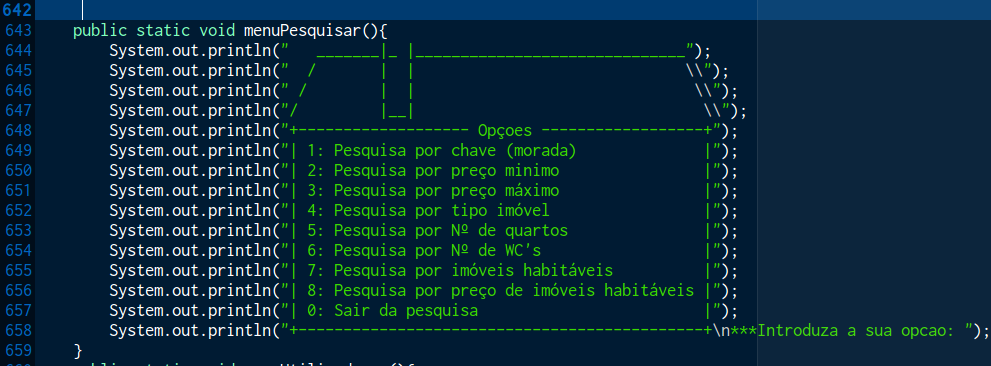
\includegraphics[scale=0.4]{002.png}	 
\newline
\newline

A interface situada na nossa classe principal com a main foi criada em Sublime Text (com a ajuda dos cursores múltiplos) em conjunto com o BlueJ e foi também utilizado ocasionalmente o IntelliJ IDEA.
\newline

Também recorremos à "Classe que abstrai a utilização da classe Scanner", criada pelo professor F. Mário Martins e a uma espécie de Feed de notícias com recurso a uma Queue que foi tirado de um tutorial.
\newline
\newline
\newline

Sem mais demoras, passaremos a uma das principais partes do nosso projeto, os imóveis.

\pagebreak

\textbf{\\Imóvel}
\newline

"Imóvel" é a primeira classe que começamos a fazer e é uma das duas classes abstratas do nosso programa, para conseguirmos criar imóveis mais específicos, neste caso, para dividi-los em diversas categorias para determinarmos variáveis extra. 
\newline

A classe é composta pelas variáveis estado, tipoImóvel, morada, precoPedido, precoMinimo e visitas. 
\newline

O clone do imóvel é ligeiramente diferente dos clones de classes normais, sendo ele:
\newline
\begin{code}

...
 abstract Imovel clone();
...

\end{code}
~\\

Também temos dois tipos de toString() diferentes (um para os vendedores e outro para os compradores, que mais tarde falaremos deles), para que possámos ocultar a informação do preço mínimo ao comprador.
\newline
\begin{code}
public String toString()\{
...
\}
\end{code}
~\\

Também existe a opção de retornar, gravar e incrementar as visitas aos nossos imóveis para uso na classe Consulta, para que quando um utilizador qualquer aceder a um dado imóvel, o sistema consiga registar esse acesso.
\newline

Imovel está também povoado pelo típico equals() muito predefinido.
\newline
\begin{code}
...
public boolean equals(Object o)\{
...
\}
...
\end{code}
~\\

Como já está praticamente tudo falado da nossa classe abstrata, iremos então descer na nossa herança para elementos menos abstratos.
\pagebreak

\textbf{"Subclasses de Imóvel"}
\newline

Comecemos com a subclasse Moradia. Esta foi a primeira subclasse que fizemos do abstract Imóvel. 
Como é habitual nas subclasses, fazemos construtores importando sempre as variáveis importantes da nossa classe abstrata através do método super(), subindo na herança para a nossa superclasse.
\newline

A subclasse Apartamento traz um tipo de variável um pouco habitual nas subclasses que fizemos que é neste caso o boolean. 
Esta subclasse também será importante para outra classe que falaremos daqui a pouco.
\newline

Tanto a classe Moradia como a classe Apartamento têm uma String em comum (Tipo). No entanto, os tipos das duas classes diferem uma da outra. Enquanto que a classe Moradia só aceita como tipos: Isolada,Germinada,Banda e Gaveto
\newline
\begin{code}

if (!tipo.equals("Isolada")&&!tipo.equals("Germinada")&&
!tipo.equals("Banda")&&!tipo.equals("Gaveto"))
{throw new TipoInvalidoException("Tipo de imóvel inválido");}

\end{code}
~\\

A subclasse Apartamento só aceita estes seguintes tipos: Simples,Duplex,Triplex
\begin{code}
if (!tipo.equals("Simples")&&!tipo.equals("Duplex")&&!tipo.equals("Triplex"))
{throw new TipoInvalidoException("Tipo de imóvel inválido");}

\end{code}
~\\

Nota: Embora fora das classes, se estas condições não forem aceites, elas irão gerar erros que mais tarde iremos falar.
\newline
\newline
\newline

A subclasse Terreno segue o mesmo príncipio das de cima, sendo o nome da String ligeiramente diferente, apropriadoPara, tal como a subclasse Loja que tem tiponegocio como nome da String.
\newline

Aqui entra a importância da Apartamento, pois uma classe Loja pode ser habitável. Ora, podemos fazer uma subclasse de Loja, ficando assim com uma subclasse LojaHabitavel, em que o principal objetivo é ligar dados do apartamento a uma dada loja.
\newline
\newline

Todas estas subclasses tem métodos em comum. Para facilitar a vida e para organização de código, nós criámos duas interfaces (Pesquisa e Habitável).
\newline
\newline

Pesquisas irá dar jeito para pesquisar o número de quartos ou o número de WC's de uma dada Moradia ou de um dado Apartamento.
\newline

Habitável por outro lado dá-nos jeito para saber se a nossa loja será habitável ou não e também retornar o preço pedido de um dado Imóvel (sendo Terreno a única exceção, a classe não tem a variável preçoPedido).    

\pagebreak

\textbf{Utilizadores}
~\\

Tivemos que implementar 3 outras classes para criar um cenário de gestão de utilizadores. 
\newline

Temos uma classe abstrata chamada Utilizador que tem outras duas subclasses ligadas a ela, sendo elas Vendedor e Comprador.
\newline

No projeto ImOObiliaria, temos 3 estados que um utilizador pode usar:
\newline
\begin{itemize}
\item Utilizador não registado
\item Vendedor registado
\item Comprador registado
\end{itemize}

O facto de um utilizador estar registado ou não depende de um simples boolean.\\ 

Esse boolean diz-nos se o utilizador em questão já passou pelo estado de registo ou não.
~\\
\newline
\begin{quote}
NOTA: quando construímos um utilizador (vendedor ou comprador) vazio, a flag registado começa sempre com o valor "false".
\end{quote}

~\\
Temos metido um apontador para a nossa principal "base de dados" (se é que podemos chamar assim). 
É também uma declaração importante na nossa superclasse que se deixássemos de lado, provavelmente não funcionaria da maneira que queriamos (é de notar que os principais métodos de procura de imóveis estão quase todas nos utilizadores).
\newline
Esse apontador é feito usando:
\newline
\begin{code}
...
    private Imobiliaria imob;
...
\end{code}
que nos permite então aceder sem problemas aos métodos principais da nossa classe Imobiliaria.
\newline
O resto das variáveis que usamos na superclasse Utilizadores é bastante normal e o básico para o funcionamento do projeto ImOObiliaria.
\newline
As subclasses tem pouco para mostrar em código, mas são extremamente precisas para que haja correta gestão dos dados.
\pagebreak

\textbf{Vendedor}
~\\
Um vendedor registado consegue ter permissões avaçandas ao programa, nomeadamente aceder ao menu exclusivo dos vendedores e a algumas opções do menu dos leilões. \\
A classe Vendedor não contém grandes operações. Tem em vez disso dois portfólios distintos: um para armazenar os imóveis que estão em venda na base de dados e outro para\\
registar os imóveis que já foram vendidos.
~\\
O vendedor também tem a possibilidade de remover diretamente um imóvel da base de dados, utilizando para isso o apontador para a classe Imobiliaria.


\textbf{Comprador}
~\\
Este estado também tem as suas únicas permissões não tão avançadas como um vendedor. Um comprador pode aceder ao menu exclusivo dos compradores, 
onde a criação, edição ou a eliminação de todos os imóveis não são permitidos.
\\
Um comprador também consegue ter acesso aos leilões. No entanto dar início a um dado leilão ou encerrar um leilão não são operações permitidas.
O comprador, ao contrário do vendedor, não tem nenhum portfólio de imóveis em venda ou vendidos mas sim uma lista de imóveis da escolha do comprador que possa gostar mais.
\\
A classe comprador é das únicas classes que recorre à ordenação de listas, recorrendo para isso às classes Comparator que estão situadas no projeto.
~\\
\newline
\begin{code}
... TreeSet <Imovel> (new ImovelStringComparator ()); ...
\end{code}
~\\
Ambas as classes recorrem ao método clone() para no caso de querermos registar informação de um dado utilizador sem alterar absolutamente nada do objeto original.


\pagebreak
%-------------------TUDO BEM POR AQUI ----------------------------------------------------------------------

\section{O motor do projeto}

\textbf{Imobiliaria (Base de dados)}
\\

Esta classe é a classe que provavelmente tem o maior número de métodos do nosso projeto (a grande responsável pela criação de dados).
\\
As variáveis de instância desta classe são as que fazem o armazenamento de grande parte dos dados dos imóveis, utilizadores e um feed de notícias . 
\\

Quase todos os nossos getters recorrem a uma lista ou map auxiliares, de forma a que retornemos corretamente os dados enquanto que os setters são práticamente normais.
\\

A classe faz-nos a gestão do inicio e do encerramento da sessão atual, não continuando se a base de dados dos utilizadores não tiver conteúdo ou se nenhuma sessão estiver ativa respetivamente.
\\
Ao iniciarmos um programa, nós temos que criar um ponto em que haja um tipo de utilizador que não seja abstrato (pois não podemos instanciar uma classe abstrata) nem esteja registado.\\
Para isso recorremos a uma maneira de simular o que queriamos, criando um método init que inicia um Comprador sem qualquer informação mas que esteja ligado à nossa base de dados, em que a flag registado seja false para não ter permissões aos nossos menus especiais.
\newline
\begin{code}
   public void init()\{atual = new Comprador ("","","","","",this,false);\}
\end{code}
~\\
Ao terminar a sessão, a classe cria um ponto de situação em que o utilizador não tem informação e não está registado no sistema (boolean registado = false;).
\newline
\begin{code}
public void fechaSessao()\{... \}
\end{code}
~\\

Os imóveis poderão ser registados, editados, listados ou removidos através desta classe, assim como os utilizadores também poderão ser registados e listados, mas não editados ou removidos.

O algoritmo do mapeamento de imóveis e do top de visitas dos imóveis também foi inserido nesta classe e recorre a apontadores dos dois tipos de utilizadores, para que possámos relacionar as visitas que os compradores ou os vendedores fazem aos imóveis, ou relacionar os vendedores e os seus respetivos imóveis em venda/reservados/vendidos.
~\\

Dois dos métodos mais importantes desta classe são os que nos permite a função de carregamento ou de salvaguarda de objetos, ou seja, guardar o estado inteiro do nosso programa.
Para isso usamos então as classes predefinidas de JAVA ObjectInputStream e ObjectOutputStream. 
~\\

\textbf{ImOObiliaria (Main)}
\newline
~\\

Este é o nosso arranque, a classe que tem o controlo dos principais menus de gestão do utilizador, de pesquisa, de vendedor e comprador, do leilão e do mapeamento de imóveis mais o top das consultas de imóveis do programa.

~\\
ImOObiliaria é a grande responsável por listar dados. No entanto, insereImovel é dos únicos métodos nesta função que utiliza o algoritmo de criação de dados em vez de listar, sendo a implementação desta função nesta classe um pouco estranha.
~\\


\pagebreak
\section{Outras classes importantes}

\textbf{Leilões}

\begin{code}

\end{code}


\pagebreak

\textbf{Aposta}

\begin{code}

\end{code}

\textbf{Consulta}

\textbf{Tempo}

\pagebreak

\section{Quando o código rebenta...}

\textbf{Exceptions}
\pagebreak

%-------------------- ISTO É UM SEPARADOR ... A SÉRIO----------------------------------------------------------------------
 
\section{Conclusão}

Principais dificuldades que não foram superadas neste projeto:

~\\
UTF-8 (utilização de caract§Ã£res especiais).
~\\
Leilões (comprador apostar de x em x minutos).
~\\
Bug estupido do double mostrar 0.0 em vez do valor devido.
~\\
Top X de imóveis não foi inteiramente implementado.
~\\

Dificuldades superadas:
~\\
fazer catch de uma exception no lugar errado...
~\\
Clone() (não dava o apontador do que queriamos)
~\\
Mapeamento de imóveis dava todos os imóveis para todos os vendedores.
~\\
Comprar um imóvel não alterava o estado do imóvel para reservado.


Este trabalho foi extremamente produtivo e só me trouxe vantagens para conhecer o mundo dos Exceptions, visto que começamos a "atinar" com eles.

\end{document}